\documentclass[tikz,border=10pt]{standalone}
\usepackage{tikz}
\usetikzlibrary{positioning}
\begin{document}
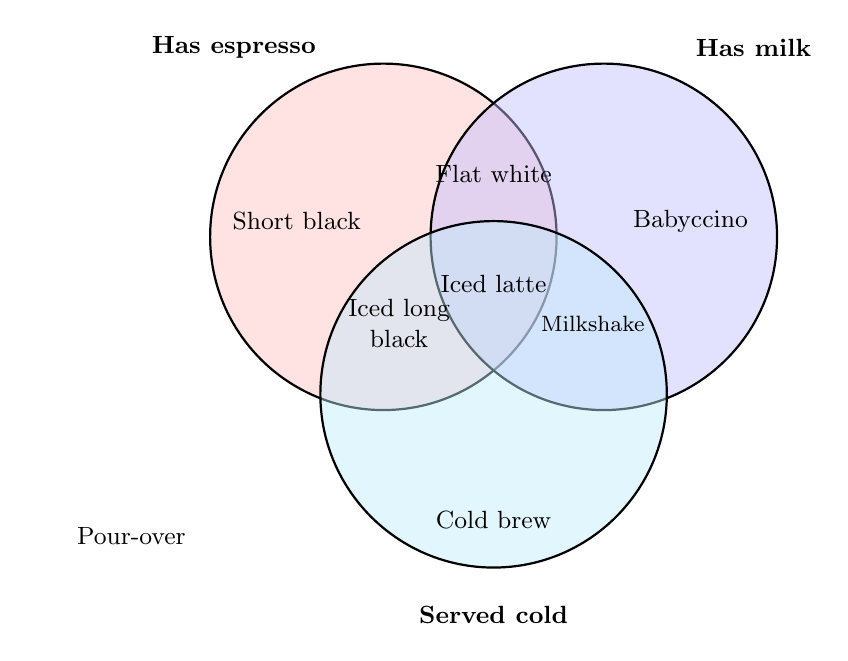
\begin{tikzpicture}[
  set/.style={circle, minimum size=4.4cm, draw=black, thick},
  item/.style={font=\small, align=center, text width=2.4cm},
]
  % Circles
  \node[set, fill=red!25, fill opacity=0.45] (E) at (-1.4,0.6) {};
  \node[set, fill=blue!25, fill opacity=0.45] (M) at (1.4,0.6) {};
  \node[set, fill=cyan!25, fill opacity=0.45] (C) at (0,-1.4) {};

  % Set labels
  \node[font=\bfseries\small] at (-3.3,3.0) {Has espresso};
  \node[font=\bfseries\small] at (3.3,3.0) {Has milk};
  \node[font=\bfseries\small] at (0,-4.2) {Served cold};

  % Drinks (each placed in the region it belongs to)
  \node[item] at (-2.5,0.8) {Short black};          % espresso only
  \node[item] at (2.5,0.8) {Babyccino};             % milk only
  \node[item] at (0,-3.0) {Cold brew};              % cold only
  \node[item] at (0,1.4) {Flat white};              % espresso + milk
  \node[item, text width=1.4cm] at (-1.2,-0.5) {Iced long black};     % espresso + cold
  \node[font=\footnotesize] at (1.26,-0.5) {Milkshake};             % milk + cold
  \node[item, text width=1.8cm] at (0,0) {Iced latte}; % all three
  \node[item] at (-4.6,-3.2) {Pour-over};           % none
\end{tikzpicture}
\end{document}
